\twocolumn
$AMNB$. Дальнейшее решение задачи не вызывает принципиальных затруднений, и мы предоставляем это читателям; искомая площадь $S = 4/\sqrt{3}$

Ещё большее внимание требуется при решении задач, в которых геометрическая конфигурация задаётся не числовыми, а буквенными дынными, т. е. в своего рода геометрических задачах с параметрами. В этих задачах ( так же, как и в алгебраических задачах с параметрами) и способ решения, и получаемый ответ могут существенно зависеть от соотношений между параметрами, определяющими конфигурацю.

Пусть, например, в разобранной только что задаче секущая плоскость проведена под углом $\phi$ к плоскости основания, а все остальные числовые данные - те же самые. Тогда в решении следует рассмотреть три случая:
\begin{enumerate}[noitemsep]
	\item Точка $M$ лежит на ребре $DD_1$;
	\item Точка $M$ совпадает с $D_1$;
	\item Точка $M$ лежит на продолжении ребра $DD_1$;
\end{enumerate}

Какой именно из указанных случаев имеет место, зависит от величины угла $\phi$, и определить это можно, исходя из сравнения отрезков $MD$ и $DD_1$. Независимо от расположения точки $M$ на прямой $DD_1$, ясно, что $MD = KD \tg{\phi} = \tg{\phi}$. Поэтому указанные случаи определяются условиями:
\begin{enumerate}[noitemsep]
	\item $\tg{\phi} < 1$;
	\item $\tg{\phi} = 1$;
	\item $\tg{\phi} > 1$;
\end{enumerate}

Таким образом, если $\phi < 45°$, то имеет место первый случай (рис. 6), и тогда $S = 2/\cos{\phi}$. Если $\phi > 45°$, то имеет место третий случай (рис. 7), тогда $S = 2/\sin{\phi}$. Что же касается случая $\phi = 45°$, то его нужно было бы рассмотреть на специальном чертеже, но фактически можно использовать и любой из имеющихся - так довольно часто бывает при рассмотрении $\ll$крайних$\gg$ значений; в этом случае $S = 2\sqrt{2}$.

Окончательный ответ записывается в виде  
\[	S =
	\begin{cases}
		2/\cos{\phi}, \text{ если} \phi < 45°, \\
		2\sqrt{2}, \text{ если} \phi = 45°,\\
		2/\sin{\phi}, \text{ если} \phi > 45°.\\
	\end{cases}
\]


Можно, разумеется, включить второй случай в любой из двух других, и записать ответ более компактно.

C аналогичной ситуацией мы встречаемся и в следующей задаче. Правда, окончательный ответ в ней от вида конфигурации не зависит и одинаков для всех значений параметра, однако промежуточные вычисления проводятся по-разному для различных конфигураций. Естественно, что решение, в котором рассмотрены не все геометрически различные случаи, не может считаться полноценным, хотя формально получается правильный ответ.


\textbf{Задача 5} (МГУ, мехмат, 1970). \textit{Шар радиуса $r$ касается плоскости $P$ в точке $A$. Прямая образует с плоскостью $P$ угол $\phi$, пересекает эту плоскость в точке $C$ и касается шара в точке $B$. Найти длину отрезка $AB$, если $AC = 2r$.}


Изобразим конфигурацию, о которой идет речь в условии (рис. 8). Из точки $B$ опустим перпендикуляр $BB_1$ на плоскость $P$ и проведем отрезок $CB_1$; ясно, что $BCB_1 = \phi$ . Далее, $OA = OB = r$, а $CB = CA =2r$ по свойству касательных к шару, проведенных из одной точки. 
\begin{figure}[h]
	\centering
	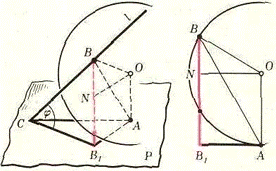
\includegraphics[width=1\linewidth]{pic_8}
	\caption{}
	\label{fig:circle}
\end{figure}
\newpage



\begin{tabular}{|c|c|c|c|c|}
\hline
ы & 0 & 1 & 2 & 3 \\
\hline
0 & 0 & 1 & 2 & 3 \\
\hline
1 & 1 & 2 & 3 & 0 \\
\hline
2 & 2 & 3 & 0 & 1 \\
\hline
3 & 3 & 0 & 1 & 2 \\
\hline
\end{tabular}
